% Drawing 74/04-12 -- folder 74, batch 04, archive page 79 (PDF page 80).
% Transcription: un cube de revêtements analogue à celui de la page 78 : $H_r$ (marqué $D_6$) $\xrightarrow{2} H_s$, $H_r \to H_{p'}$ (marqué $\mathfrak{S}_3$), $H_{s^*}$, $H_d$ (flèches « opp » et 2), $H_{trr}$, $H_{tr}$ (marqué $\mathbb{F}_2^2$), $H_\omega$, $H_{tr^*}$, $e$ ; flèches verticales de degré 3, les autres de degré 2. À gauche, un petit hexagone à triangles inscrits en pointillés.
% Kind: cube of coverings (arrow diagram), small hexagon. Method 2 (schematic redraw from the facsimile). Status: partial.
% Notes: H_r (D_6) -2-> H_s; H_r -> H_p' (S_3 below it), H_r -> H_s* (2), H_r -> H_tr (3, vertical); H_p' -> H_d (2) and H_s* -> H_d (2, « opp »); H_s -> H_trr, H_p' -> H_omega and H_s* -> H_tr* (3, vertical); H_d -> e (3); H_tr -> H_trr, H_omega, H_tr* (2); H_trr, H_omega, H_tr* -> e (2). Labels at \small (the figure drawn at 1.6 mm per unit), placed where they stand; the vertical arrows of degree 3, the others 2. Left: a small hexagon with its two inscribed triangles dotted. Struck out and omitted: an « H_r » struck at the left of H_s, and a struck word under « opp ». Still differs: the subscripts at the centre (H_p', H_s*, H_trr) are overinked and read as in the transcription; which of the arrows from the top row end at H_p' or at H_d is partly a reading. Redrawn 2026-11-09 (issue 128): to check again.
% Coordinates: 1 unit = 1.6 mm = 1/100 of the crop width (bbox in page fractions: [0.15, 0.5, 0.6, 0.635]).
% Redrawn by Claude (claude-opus-5-5), issue #73, 2026-11-09; not checked by a human; not compiled (no TeX in the session).
% Rights: reproduces part of the work -- behind RENDER_TRANSCRIPTS, never published by itself.
\documentclass[tikz,border=3pt]{standalone}
\usepackage{amsmath,amssymb}
\usetikzlibrary{patterns,arrows.meta}
\tikzset{pencil/.style={black!45}, struck/.style={black!35}, mark/.style={circle,draw,inner sep=1.3pt}, pt/.style={circle,fill,inner sep=0.9pt}, opt/.style={circle,draw,fill=white,inner sep=1.1pt}}
\begin{document}
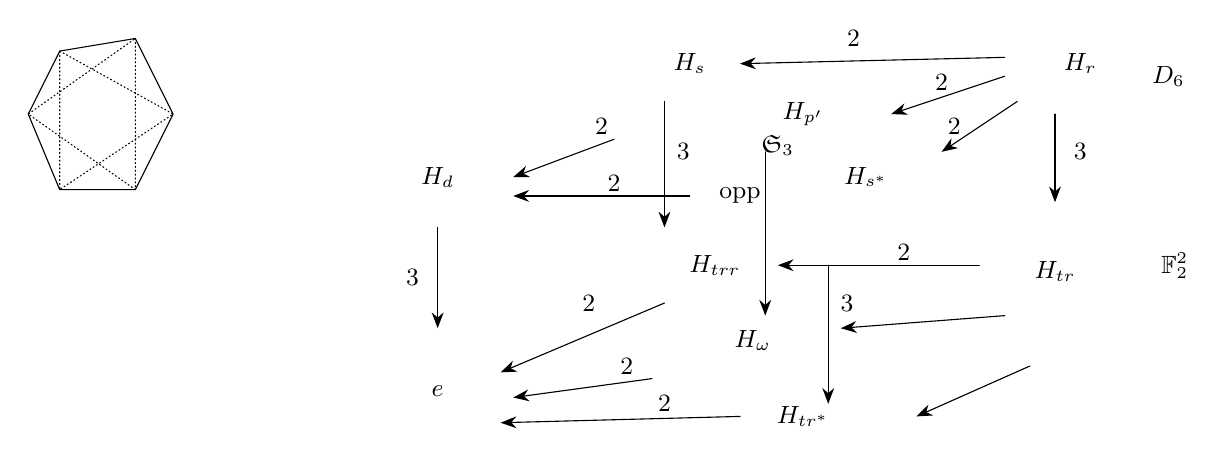
\begin{tikzpicture}[x=1.6mm,y=1.6mm,line cap=round,line join=round,font=\scriptsize]
\node[inner sep=1pt] at (53,-6) {\small $H_s$};
\draw[-{Stealth[length=2mm]}] (78,-5.5) -- (57,-6);
\node[inner sep=1pt] at (66,-4) {\small $2$};
\draw[-{Stealth[length=2mm]}] (78,-7) -- (69,-10);
\node[inner sep=1pt] at (73,-7.5) {\small $2$};
\node[inner sep=1pt] at (60,-12.5) {\small $\mathfrak S_3$};
\draw[-{Stealth[length=2mm]}] (79,-9) -- (73,-13);
\node[inner sep=1pt] at (74,-11) {\small $2$};
\node[inner sep=1pt] at (33,-15) {\small $H_d$};
\draw[-{Stealth[length=2mm]}] (47,-12) -- (39,-15);
\node[inner sep=1pt] at (46,-11) {\small $2$};
\draw[-{Stealth[length=2mm]}] (53,-16.5) -- (39,-16.5);
\node[inner sep=1pt] at (47,-15.5) {\small $2$};
\node[inner sep=1pt] at (57,-16.5) {\small opp};
\node[inner sep=1pt] at (55,-22) {\small $H_{trr}$};
\draw[-{Stealth[length=2mm]}] (76,-22) -- (60,-22);
\node[inner sep=1pt] at (70,-21) {\small $2$};
\node[inner sep=1pt] at (58,-28) {\small $H_\omega$};
\node[inner sep=1pt] at (62,-34) {\small $H_{tr^*}$};
\node[inner sep=1pt] at (33,-32) {\small $e$};
\draw[-{Stealth[length=2mm]}] (51,-25) -- (38,-30.5);
\node[inner sep=1pt] at (45,-25) {\small $2$};
\draw[-{Stealth[length=2mm]}] (50,-31) -- (39,-32.5);
\node[inner sep=1pt] at (48,-30) {\small $2$};
\draw[-{Stealth[length=2mm]}] (57,-34) -- (38,-34.5);
\node[inner sep=1pt] at (51,-33) {\small $2$};
\draw[-{Stealth[length=2mm]}] (80,-30) -- (71,-34);
\draw[-{Stealth[length=2mm]}] (78,-26) -- (65,-27);
\draw[-{Stealth[length=2mm]}] (33,-19) -- (33,-27);
\node[inner sep=1pt] at (31,-23) {\small $3$};
\draw[-{Stealth[length=2mm]}] (51,-9) -- (51,-19);
\node[inner sep=1pt] at (52.5,-13) {\small $3$};
\draw[-{Stealth[length=2mm]}] (82,-10) -- (82,-17);
\node[inner sep=1pt] at (84,-13) {\small $3$};
\draw[-{Stealth[length=2mm]}] (64,-22) -- (64,-33);
\node[inner sep=1pt] at (65.5,-25) {\small $3$};
\draw (3,-5) -- (9,-4) -- (12,-10) -- (9,-16) -- (3,-16) -- (0.5,-10) -- cycle;
\draw[densely dotted] (3,-5) -- (12,-10) -- (3,-16) -- cycle;
\draw[densely dotted] (9,-4) -- (9,-16) -- (0.5,-10) -- cycle;
\node[inner sep=1pt] at (84,-6) {\small $H_r$};
\node[inner sep=1pt] at (91,-7) {\small $D_6$};
\node[inner sep=1pt] at (62,-10) {\small $H_{p'}$};
\node[inner sep=1pt] at (67,-15) {\small $H_{s^*}$};
\node[inner sep=1pt] at (82,-22.5) {\small $H_{tr}$};
\node[inner sep=1pt] at (91.5,-22) {\small $\mathbb F_2^2$};
\draw[-{Stealth[length=2mm]}] (59,-13) -- (59,-26);
\end{tikzpicture}
\end{document}
